\newpage
\section{Хөгжүүлэлтийн орчин бүрдүүлэлт}

Өмнө системийн шинжилгээ хэсэгт тодорхойлсон системийн шаардлагуудыг хэрэгжүүлэх
үүднээс өмнө судалсан технологиудын дагуу хөгжүүлэлтийн орчинг бэлдсэн.

Docker Desktop суулган дараах container-үүдийг үүсгэсэн.
\begin{figure}[H]
    \centering
    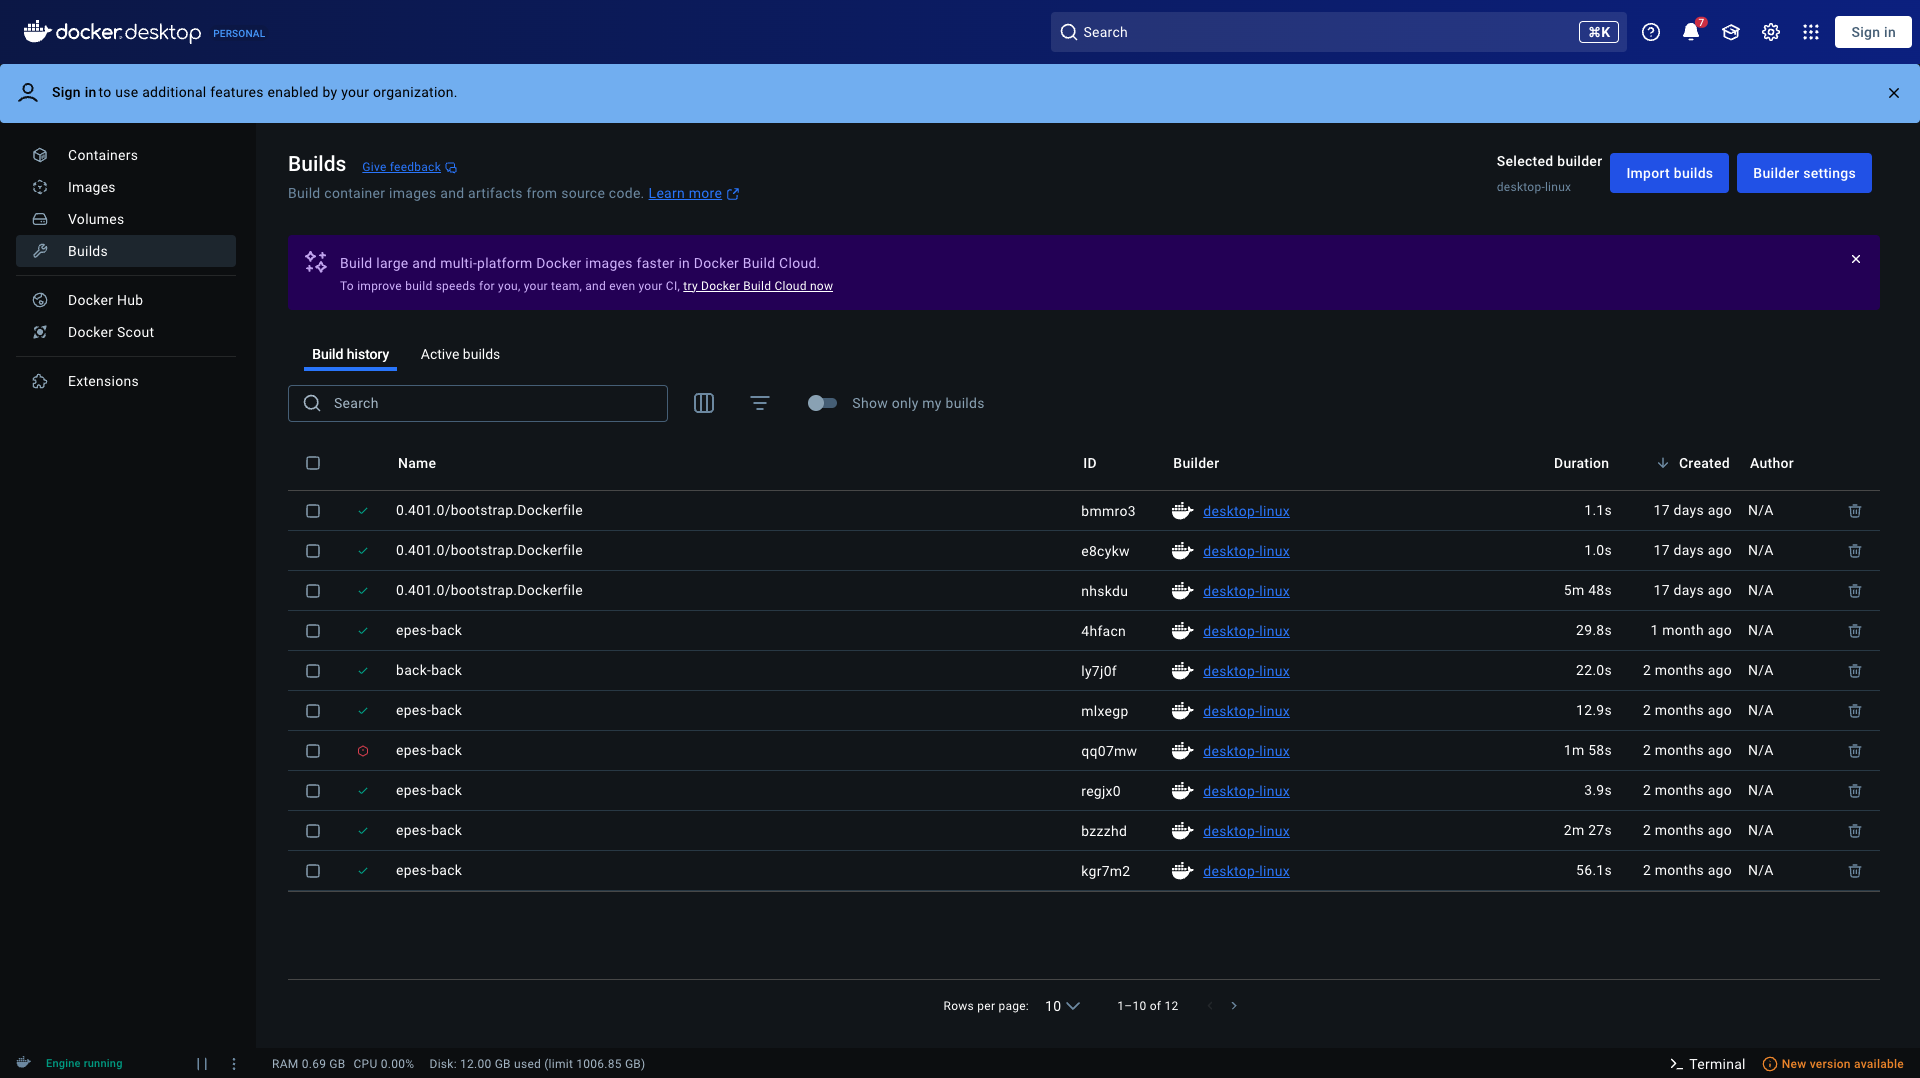
\includegraphics[scale=0.25]{src/images/uiux/dockerdash.png}
    \caption{Docker Desktop програмын интерфэйс}
    \label{fig:dockerdash}
\end{figure}

\subsection{Docker container ашиглан өгөгдлийн сан үүсгэж, түүний серверийг ажилуулахад ашигласан.}

\begin{lstlisting}[language=Docker, caption=Dockerfile, frame=single]
    FROM golang:1.24

    WORKDIR /app

    COPY go.mod go.sum ./
    RUN go mod download

    COPY . .

    RUN go build -o main .

    EXPOSE 8080

    CMD ["./main"]
\end{lstlisting}

\begin{lstlisting}[language=Docker, caption=docker-compose.yaml, frame=single]
    version: "3.8"
    services:
      app:
        build: .
        ports:
          - "8080:8080"
        depends_on:
          - db
        environment:
          - DB_HOST=db
          - DB_USER=root
          - DB_PASSWORD=rootpass
          - DB_NAME=epes_db
          - DB_PORT=5432
    
      db:
        image: postgres:latest
        environment:
          - POSTGRES_USER=root
          - POSTGRES_PASSWORD=rootpass
          - POSTGRES_DB=epes_db
        ports:
          - "5432:5432"
        volumes:
          - postgres_data:/var/lib/postgresql/data
    
    volumes:
      postgres_data:    
\end{lstlisting}

\subsection{Github орчин бүрдүүлэлт}
Github-д repo үүсгэж түүндээ системийн кодыг байршуулсан. \url{https://github.com/amgaland/epes}
Ингэснээр системид version control хийх боломжтой болсон.

\subsection{Front-end орчин бүрдүүлэлт}
Front-end хэсэгт Nextjs болон Shadcn UI болон Bun ашигласан.
\begin{lstlisting}[language=zsh, caption=Bun суулгах, frame=single]
    curl -fsSL https://bun.sh/install | bash
\end{lstlisting}

\begin{lstlisting}[language=zsh, caption=Nextjs суулгах, frame=single]
    bun install next@latest
\end{lstlisting}

\begin{lstlisting}[language=zsh, caption=Shadcn суулгах, frame=single]
    bunx --bun shadcn@latest init
\end{lstlisting}

\subsection{Back-end орчин бүрдүүлэлт}
Back-end хэсэгт golang болон gin framework ашигласан. Golang-ийг \url{https://golang.org/dl/} хаягаас татаж суулгаж болно.
\begin{lstlisting}[language=zsh, caption=Golang суулгах, frame=single]
    brew install go
    brew install gin
\end{lstlisting}

Хэрэгцээт технологиудаа суулгасны дараа шаардлагад тодорхойлсон архитектурын дагуу код бичнэ.
\subsection{Test орчин бүрдүүлэлт}

Back-end хэсгийн тестийг Postman ашиглан хийсэн. Postman-д системийн API-уудыг тестлэх орчин бүрдүүлсэн.

\begin{figure}[H]
    \centering
    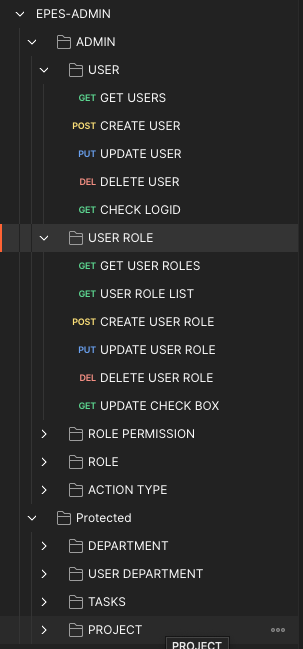
\includegraphics[scale=0.5]{src/images/uiux/postmanStruc.png}
    \caption{Postman файлын бүтэц}
    \label{fig:postman_file_struct}
\end{figure}

\subsubsection{Хэрэглэгч үүсгэх тестийн жишээ}

\begin{figure}[H]
    \centering
    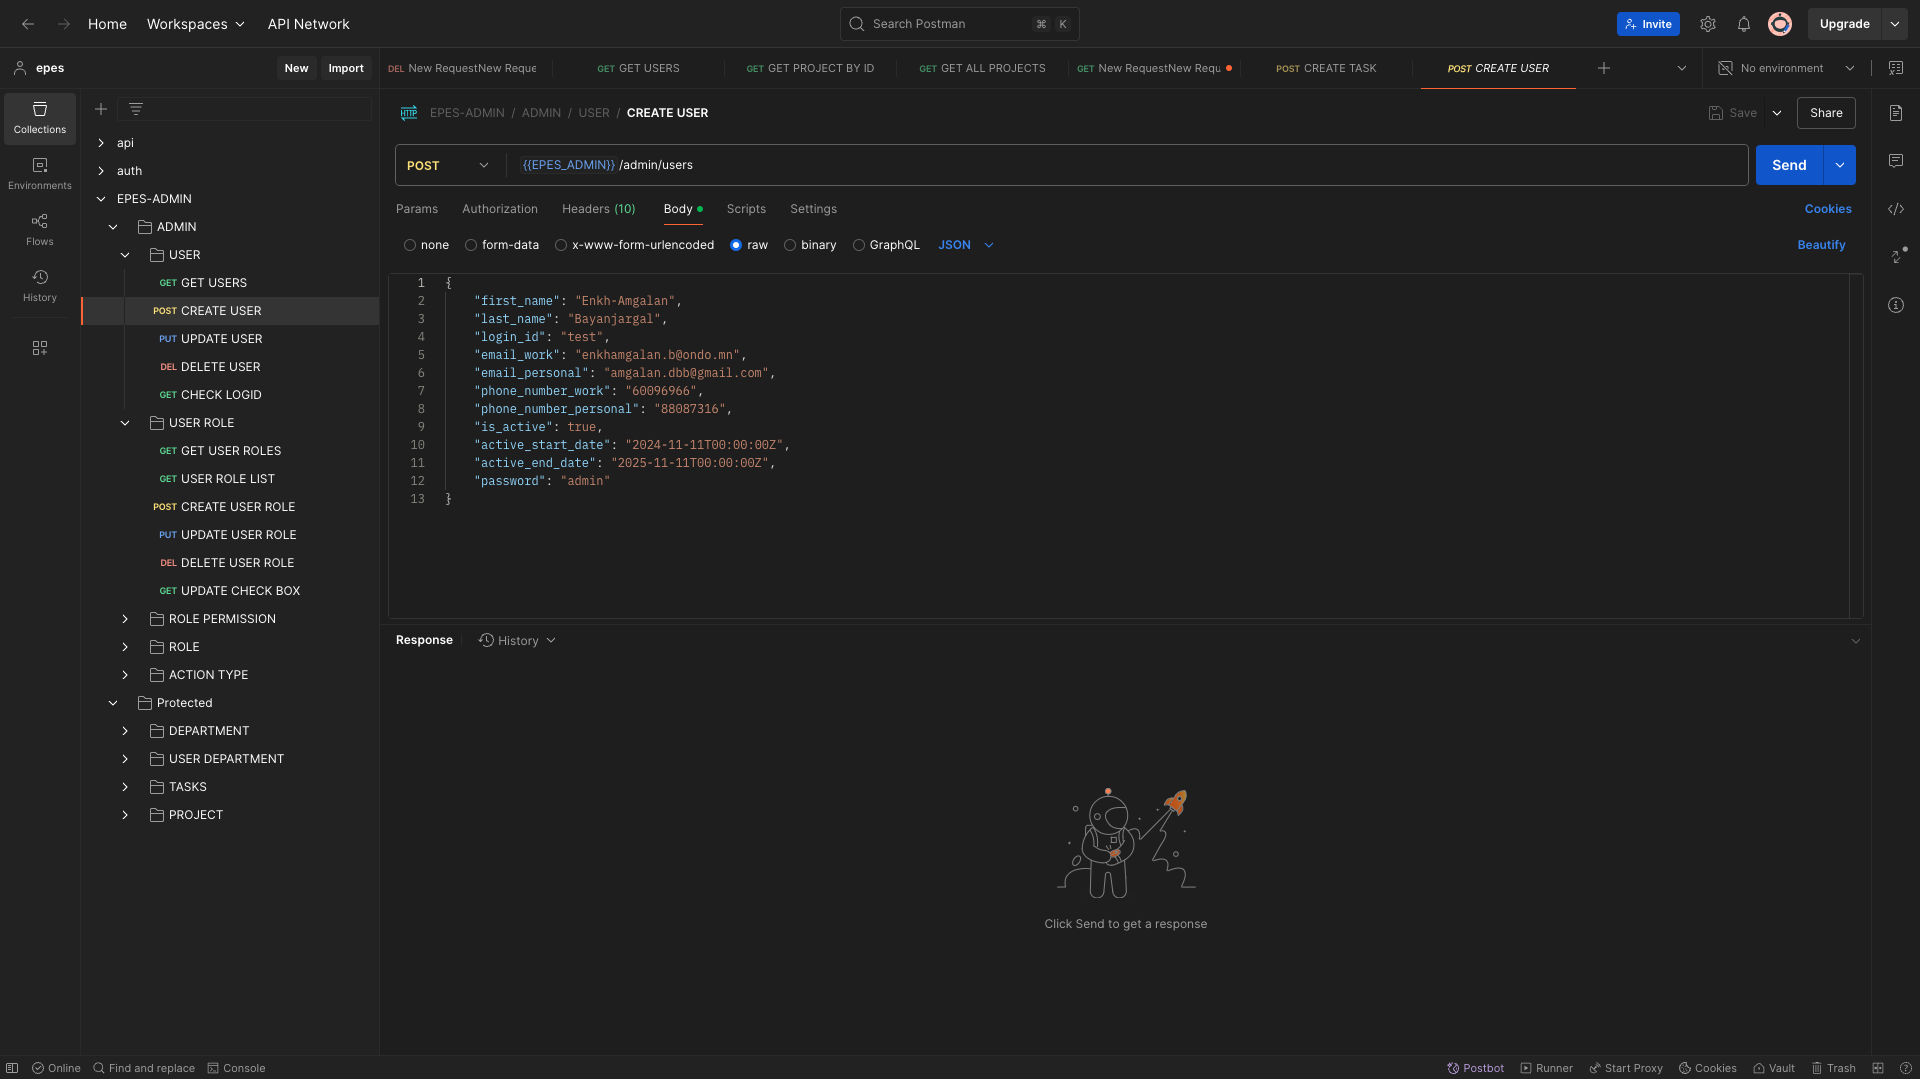
\includegraphics[scale=0.25]{src/images/uiux/postmanCreateUser.png}
    \caption{Postman хэрэглэгч үүсгэх тест}
    \label{fig:postman_create_user}
\end{figure}